\documentclass[11pt, a4paper]{article}
\usepackage[margin=1.8cm]{geometry} % permet de faire les marges personnalisées 
\usepackage{graphicx} % permet d'insérer des photos 
\usepackage{hyperref} % permet de faire des liens cliquables 

\usepackage{tabularx} % permet d'effectuer les aspects avec les dates puis les formations etc... 

\hypersetup{
    colorlinks=true,
    urlcolor=black,
    linkcolor=black
}


\pagestyle{empty} % supprime les numéros en bas de page

\begin{document}

% Bloc titre à centrer 
\noindent
\begin{minipage}[c]{1cm}
    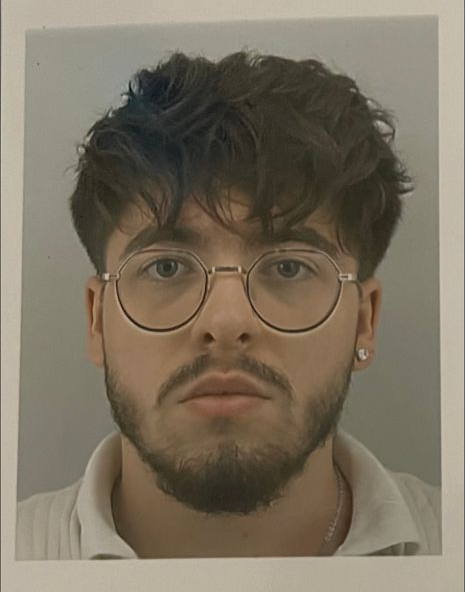
\includegraphics[width=2.5cm]{photo_identite_Lorenzo.png}
\end{minipage}
\hfill
\begin{minipage}[c]{0.75\textwidth}
\centering
{\LARGE \textbf{DERREZ Lorenzo}}\\
+33 7 50 69 25 61 \quad | \quad \href{mailto:lrdrz.professionnel@gmail.com}{lrdrz.professionnel@gmail.com} \quad | \quad \href{https://www.linkedin.com/in/lorenzo-derrez}{LinkedIn} \quad | \quad \href{https://github.com/Nmrodd}{GitHub}
\end{minipage}
\hfill
\begin{minipage}[c]{1cm}
\end{minipage}

\begin{flushleft} % permet d'insérer du text à gauche 
    \large \textit{Computer Engineering Student at ENSEIRB-MATMECA, Bordeaux}
    \\
    \small Curious, Collaborative, Rigorous, Disciplined, Detail-oriented
\end{flushleft}

\rule{\textwidth}{0.4pt}  % permet de tracer le trait 

\section*{Education} % * permet d'enlever le comportement automatique de numérotation 

\begin{tabularx}{\textwidth}{@{}l X r@{}}
    2021 --  2024 & \textbf{Lycée Beau-Jardin / Baccalauréat} \quad \textit{Saint-Dié-des-Vosges}
    \\
    & \small French Baccalaureate, with Highest Honors -- Specializations: Mathematics, Computer Science, Physics-Chemistry & \\[4pt]
    2024 -- 2026 & \textbf{Intensive Preparatory Programme for Competitive Engineering School Entrance Exams / Lycée Henri-Poincaré} \quad \textit{Nancy}
    \\
    2026 -- 2029 & \textbf{Engineering Degree, ENSEIRB-MATMECA} \quad \textit{Bordeaux}
\end{tabularx}

\vspace{2pt}
\rule{\textwidth}{0.4pt}  % permet de tracer le trait 

\section*{Experience}

\subsection*{Skills}

\begin{tabularx}{\textwidth}{@{}l X r@{}}
    \textbf{C} -- 3 years
    \\
    \textbf{Python} -- 3 years
    \\
    \textbf{OCamL} -- 2 years
    \\
    \textbf{LaTex, Vim} -- 1 year
    \\
    \\
    \textbf{French} -- Native
    \\
    \textbf{English} -- C2
    \\
    \textbf{Italian} -- B2
\end{tabularx}

\vspace{2pt}
\rule{\textwidth}{0.4pt}  % permet de tracer le trait 

\subsection*{Internships}

\begin{tabularx}{\textwidth}{@{}l X r@{}}
    2022 & \textbf{Numalliance} \quad \textit{Automated Machinery Manufacturer}
    \\
    2024 & \textbf{EY Luxembourg} \quad \textit{Cybersecurity Department}
\end{tabularx}

\vspace{2pt}
\rule{\textwidth}{0.4pt}  % permet de tracer le trait 

\subsection*{Language Immesion}

\begin{tabularx}{\textwidth}{@{}l X r@{}}
    2019 & \textbf{London} \quad \textit{European Section}
    \\
    2023 & \textbf{San Francisco} \quad \textit{English-language immersion during final year of secondary school}
    \\
    2023 & \textbf{Italie} \quad \textit{Italian language courses}
\end{tabularx}

\vspace{2pt}
\rule{\textwidth}{0.4pt}  % permet de tracer le trait 

\subsection*{Community Involvment}

\begin{tabularx}{\textwidth}{@{}l X r@{}}
    -- Active member of student associations across several educational institutions
    \\
    -- Participated in community and environmental clean-up initiatives 
    \\
    -- Organized Armistice Day commemorative events
    \\
    -- Contributed to community improvement projects organized by local municipalities 

\end{tabularx}

\vspace{2pt}
\rule{\textwidth}{0.4pt}  % permet de tracer le trait 

\subsection*{Interests and Activities}

\begin{tabularx}{\textwidth}{@{}l X r@{}}
    -- \textbf{Basket-ball} \quad \textit{Played at club level for 10 years}
    \\
    -- \textbf{Strength Training} \quad \textit{Self-directed}
    \\
    -- \textbf{Boxing} \quad \textit{Self-directed}
\end{tabularx}

\end{document}